% uklad dokumentu
	\documentclass{article}
	\usepackage{xparse}
	\usepackage[margin=1.5cm]{geometry}
    \usepackage{enumerate} 
	\frenchspacing
    \linespread{1.0}
    \setlength{\parindent}{0pt}

% jezyk polski
	\usepackage[T1]{fontenc}
	\usepackage[polish]{babel}
	\usepackage[utf8]{inputenc}
 
% pakiety matematyczne
    \let\lll\undefined
    \usepackage{mathtools}
	\usepackage{amssymb}
    \usepackage{amsthm}
	\usepackage{amsmath}
	\usepackage{amsfonts}
	\usepackage{tikz}

	\usepackage{float}	
	
% pakiety do automatów
	\usetikzlibrary{automata, arrows.meta, positioning, arrows}
	
% wykresiki
	\usepackage{pgfplots}
	\pgfplotsset{compat = newest}
	\usepackage{graphicx}
	\usepackage{subcaption}

    \title{\textbf{Algorytmy Metaheurystyczne\\Komiwojażer Heurystycznie}}
    \author{Gabriel Budziński(254609)\\Franciszek Stepek (256310)}
    \date{}
    
    
\begin{document} 
\maketitle

\section*{Przedmowa}
Na samym początku omówimy po krótce użyte algorytmy, oraz zastanowimy się nad ich złożonością obliczeniową, natomiast dalej dopiero przejdziemy do opisu eksperymentów.

\section{Podsumowanie złożoności obliczeniowych implementacji}

\section{Opis eksperymentów}
\subsection{Implementacja}
Algorytmy implementujemy w języku \texttt{C/C++}, odległości między wierzchołkami są przechowywane jako pełne tablice dwuwymiarowe typu \texttt{int}, a trasy są w kontenerach \texttt{vector}, co ułatwia operacje odwracania i mieszania.\\
Korzystaliśmy z kompilatora g++ wraz z użyciem flag -lSDL2 (używanej przy wizualizacji, wraz z odpowiednim dla danego systemu operacyjnego podlinkowania do folderu zawierającego) oraz -lpthread (przy korzystaniu z wielowątkowości)

\subsection{Sprzęt}
Programy były testowane na dwóch maszynach, laptopie \textit{Lenovo} i komputerze stacjonarnym. Obie jednostki są wyposażone w procesor architektury \texttt{x86} marki \texttt{intel} oraz 16GB pamięci RAM.

\subsubsection{Pececik}
Komputer stacjonarny posiada procesor sześciordzeniowy i5-10600K 4,1 GHz (o obniżonym napięciu operacyjnym).
\subsubsection{Lapek}
Laptop posiada procesor czterordzeniowy i7-6700HQ 2,6 GHz

\subsection{Instancje}
\subsubsection{Przykłady TSPLIB}
W części eksperymentów użyto instancji euklidejskiego problemu komiwojażera.

\subsubsection{Instancje losowe}
W celu zwiększenia liczności i dokładności testów spreparowano losowo generowane instancje eukidejskiego problemu komiwojażera.

\subsection{Metodologia/cel}

Testy przeprowadzono za pomocą zaimplementowanych w tym celu funkcji ku jak największej automatyzacji. Dane o przeprowadzonych testach zapisywano do plików tekstowych w formacie CSV, a następnie poddane analizie. Testowanie miało na celu wskazanie mocnych i słabych stron zaimplementowanych heurystyk, jak i ich porównanie.

\subsection{Opis wyników}

\subsection{Porównanie wariantów dla optymalnych parametrów}

Po przetestowaniu optymalnych parametrów przeprowadzono testy dla ustalonych instancji TSPLIB. Wykresy podzielono na dwie grupy, po lewej operacja \texttt{kick} była losowa w zadanym przedziale, po prawej deterministyczna.
\\

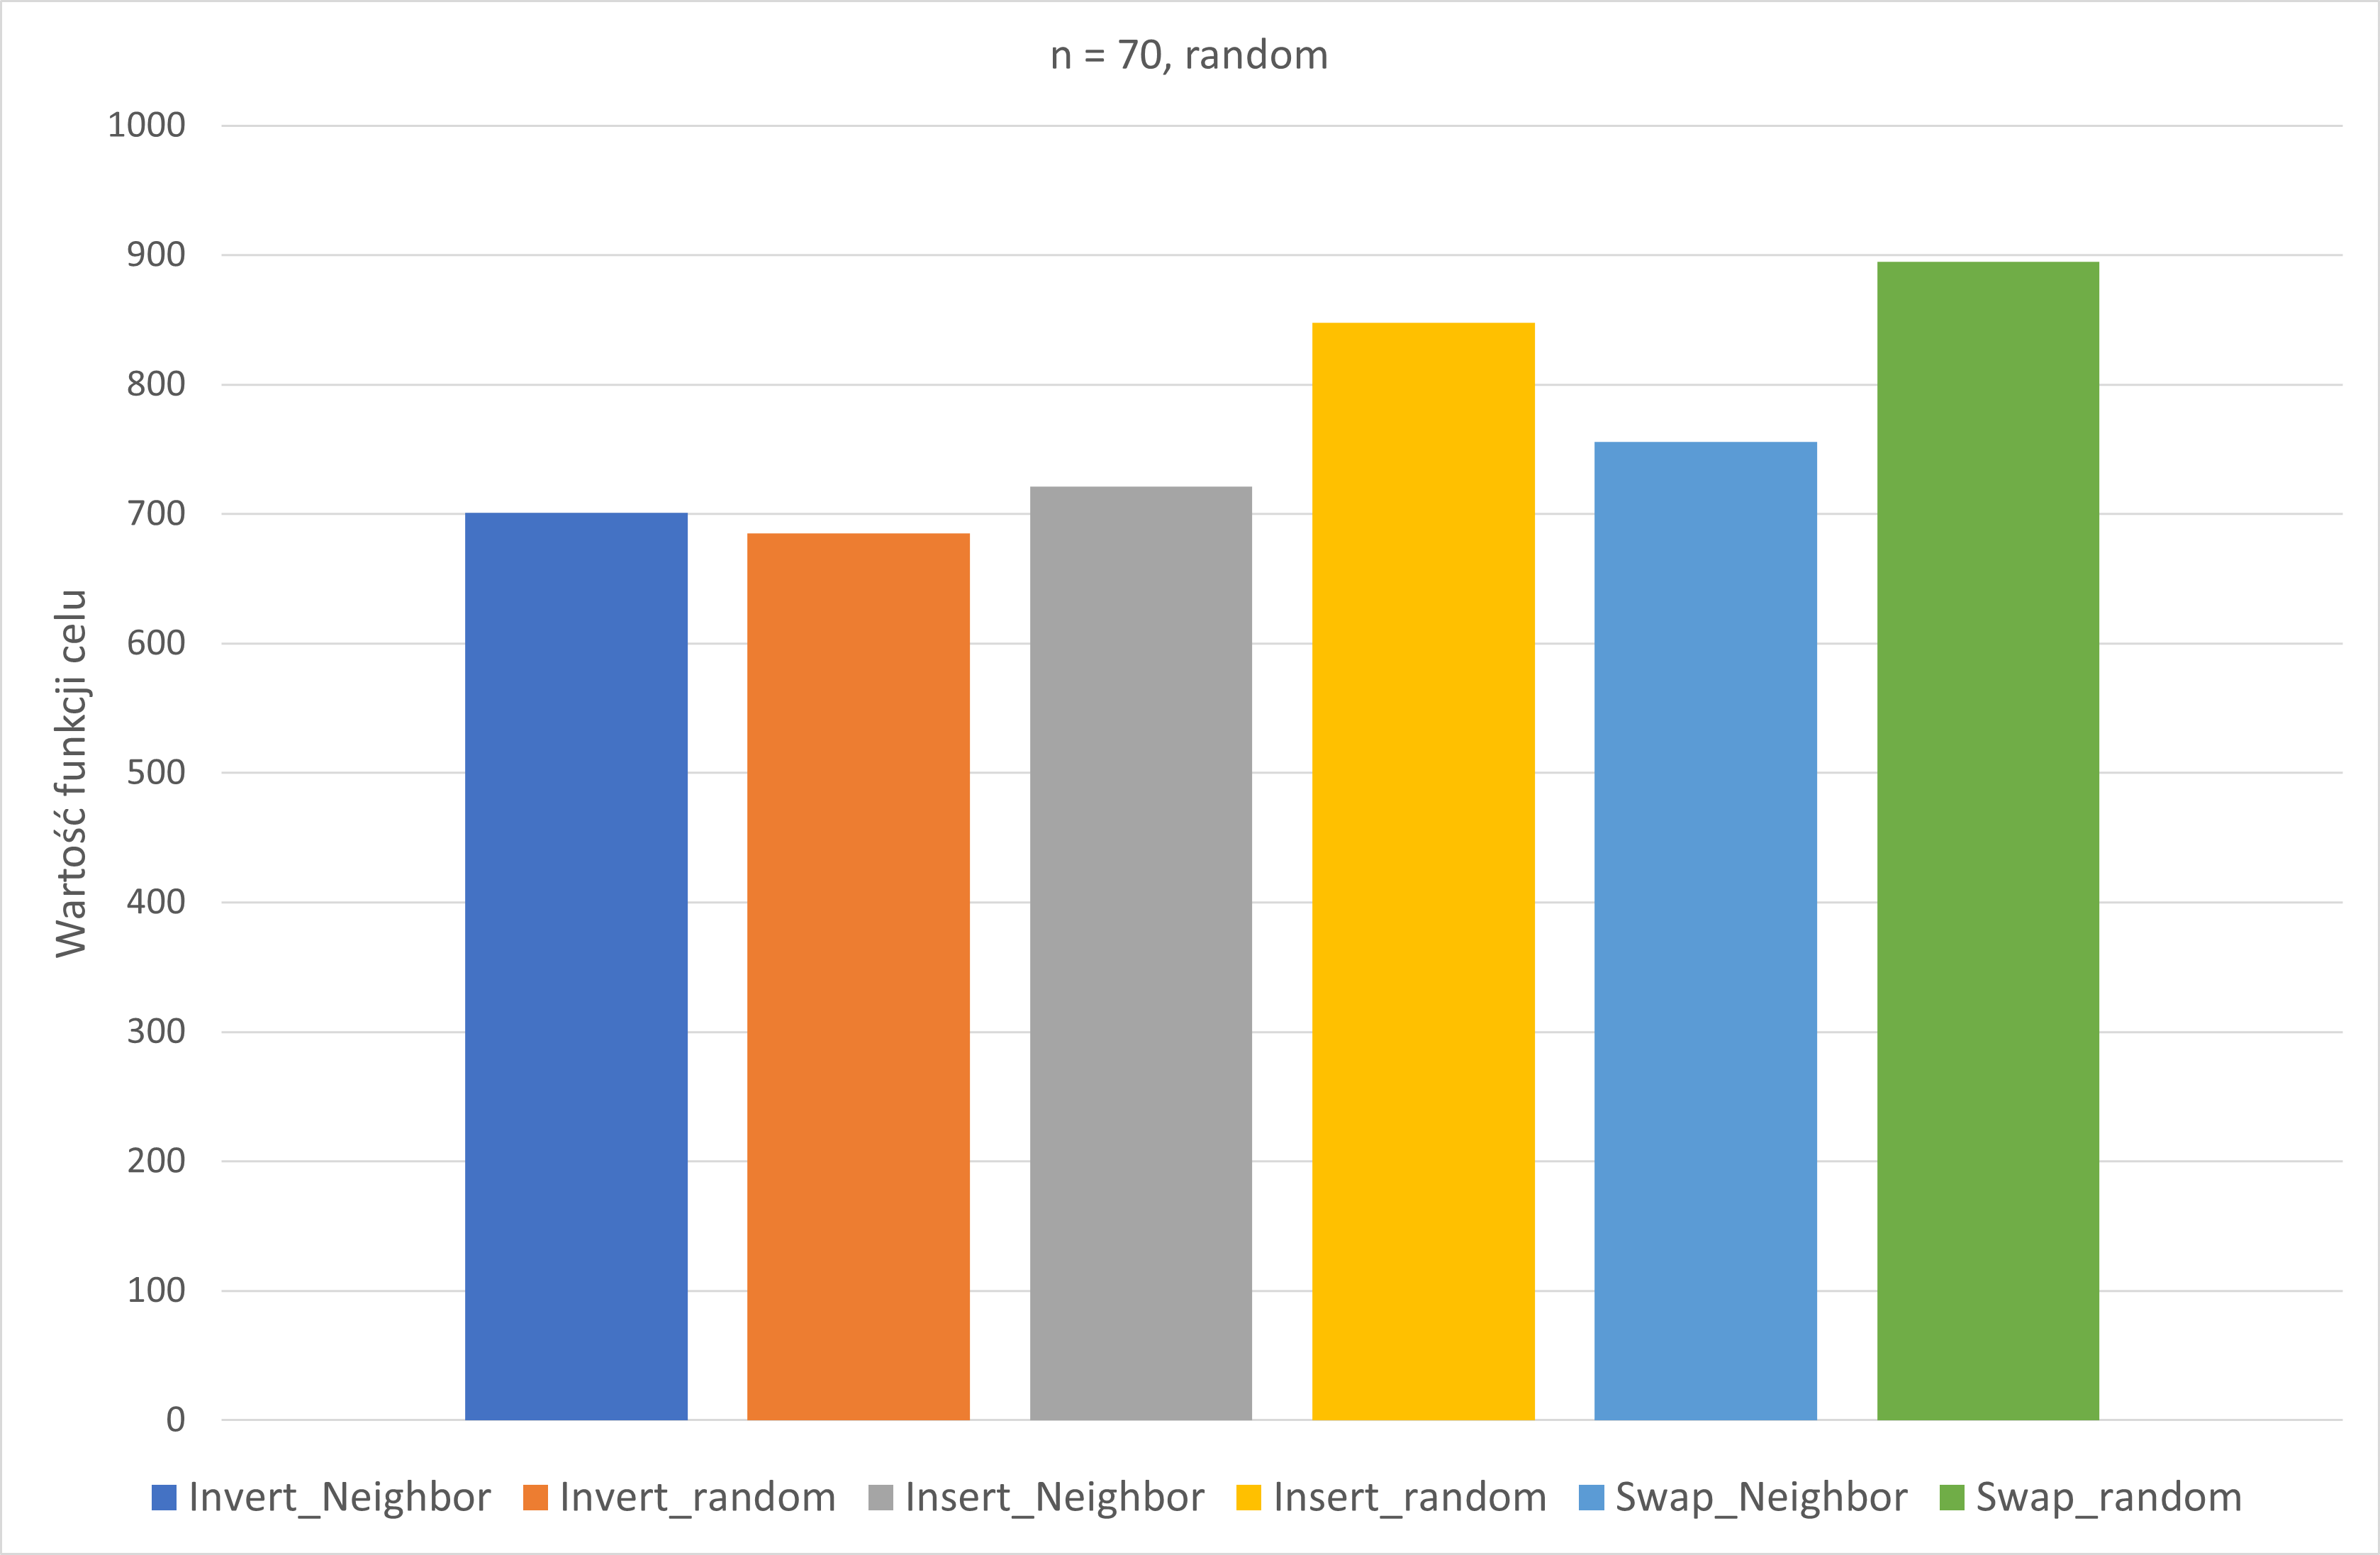
\includegraphics[scale=0.36]{70_rand}
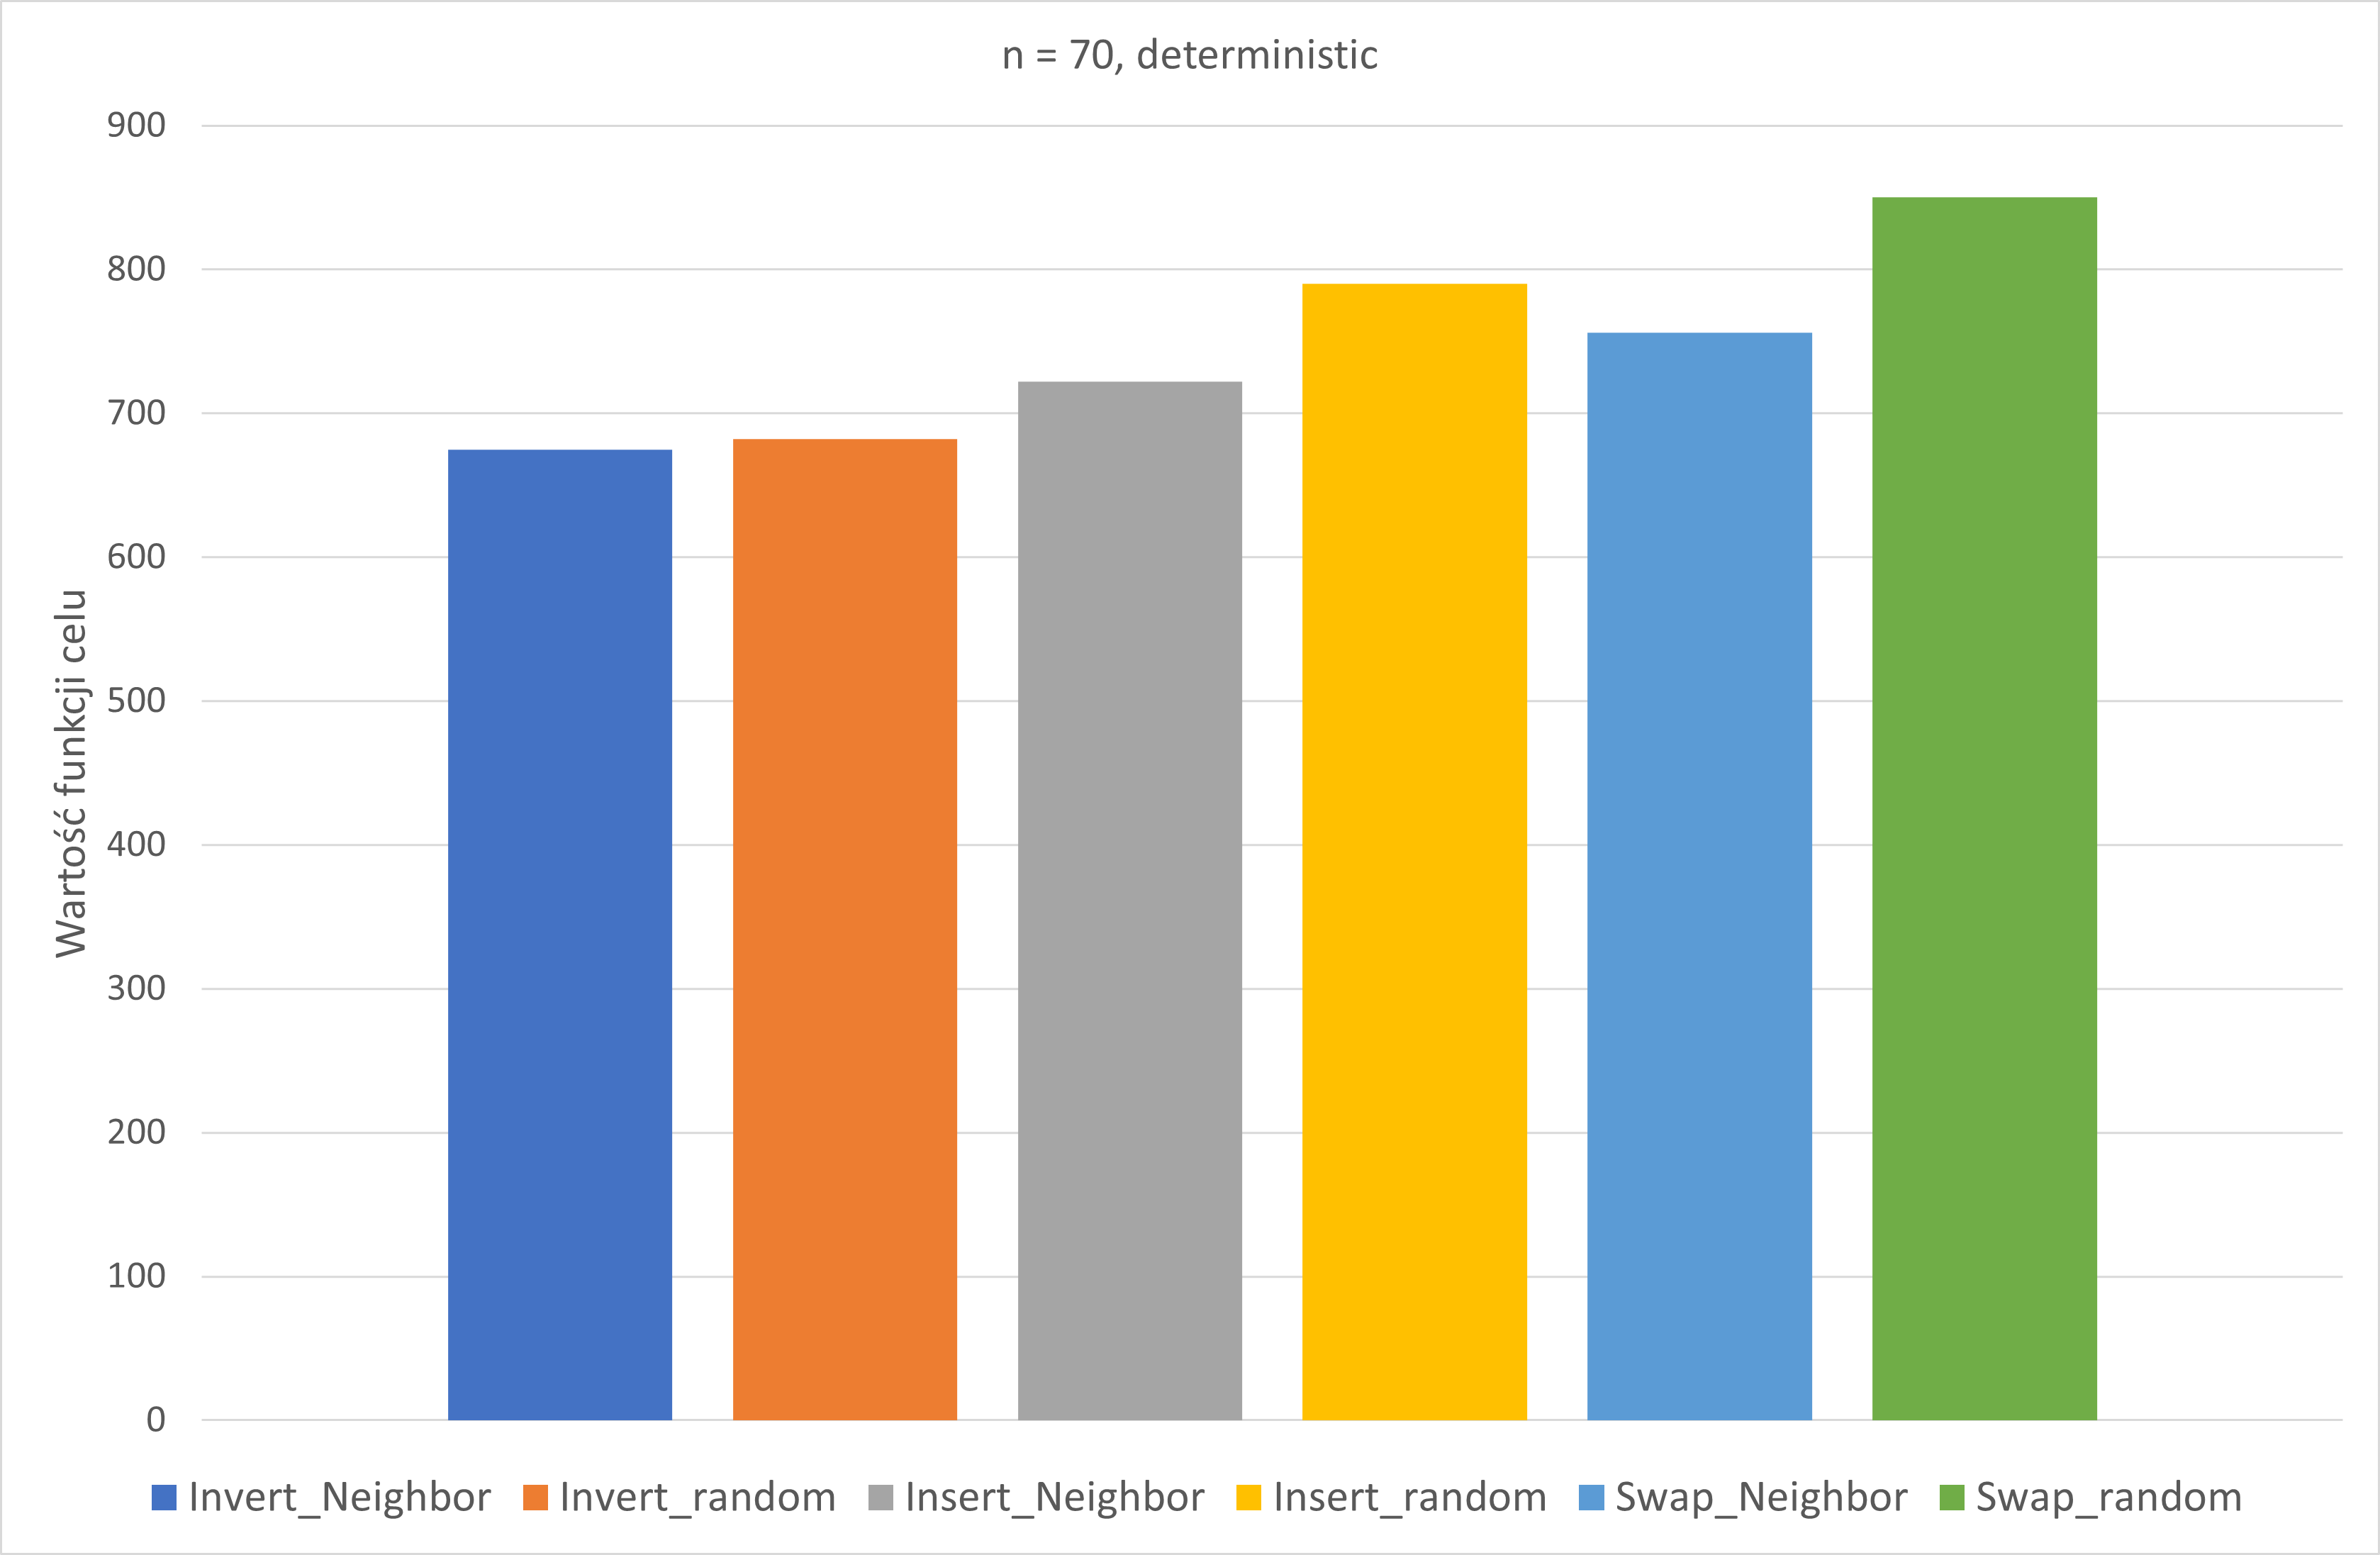
\includegraphics[scale=0.36]{70_deter}
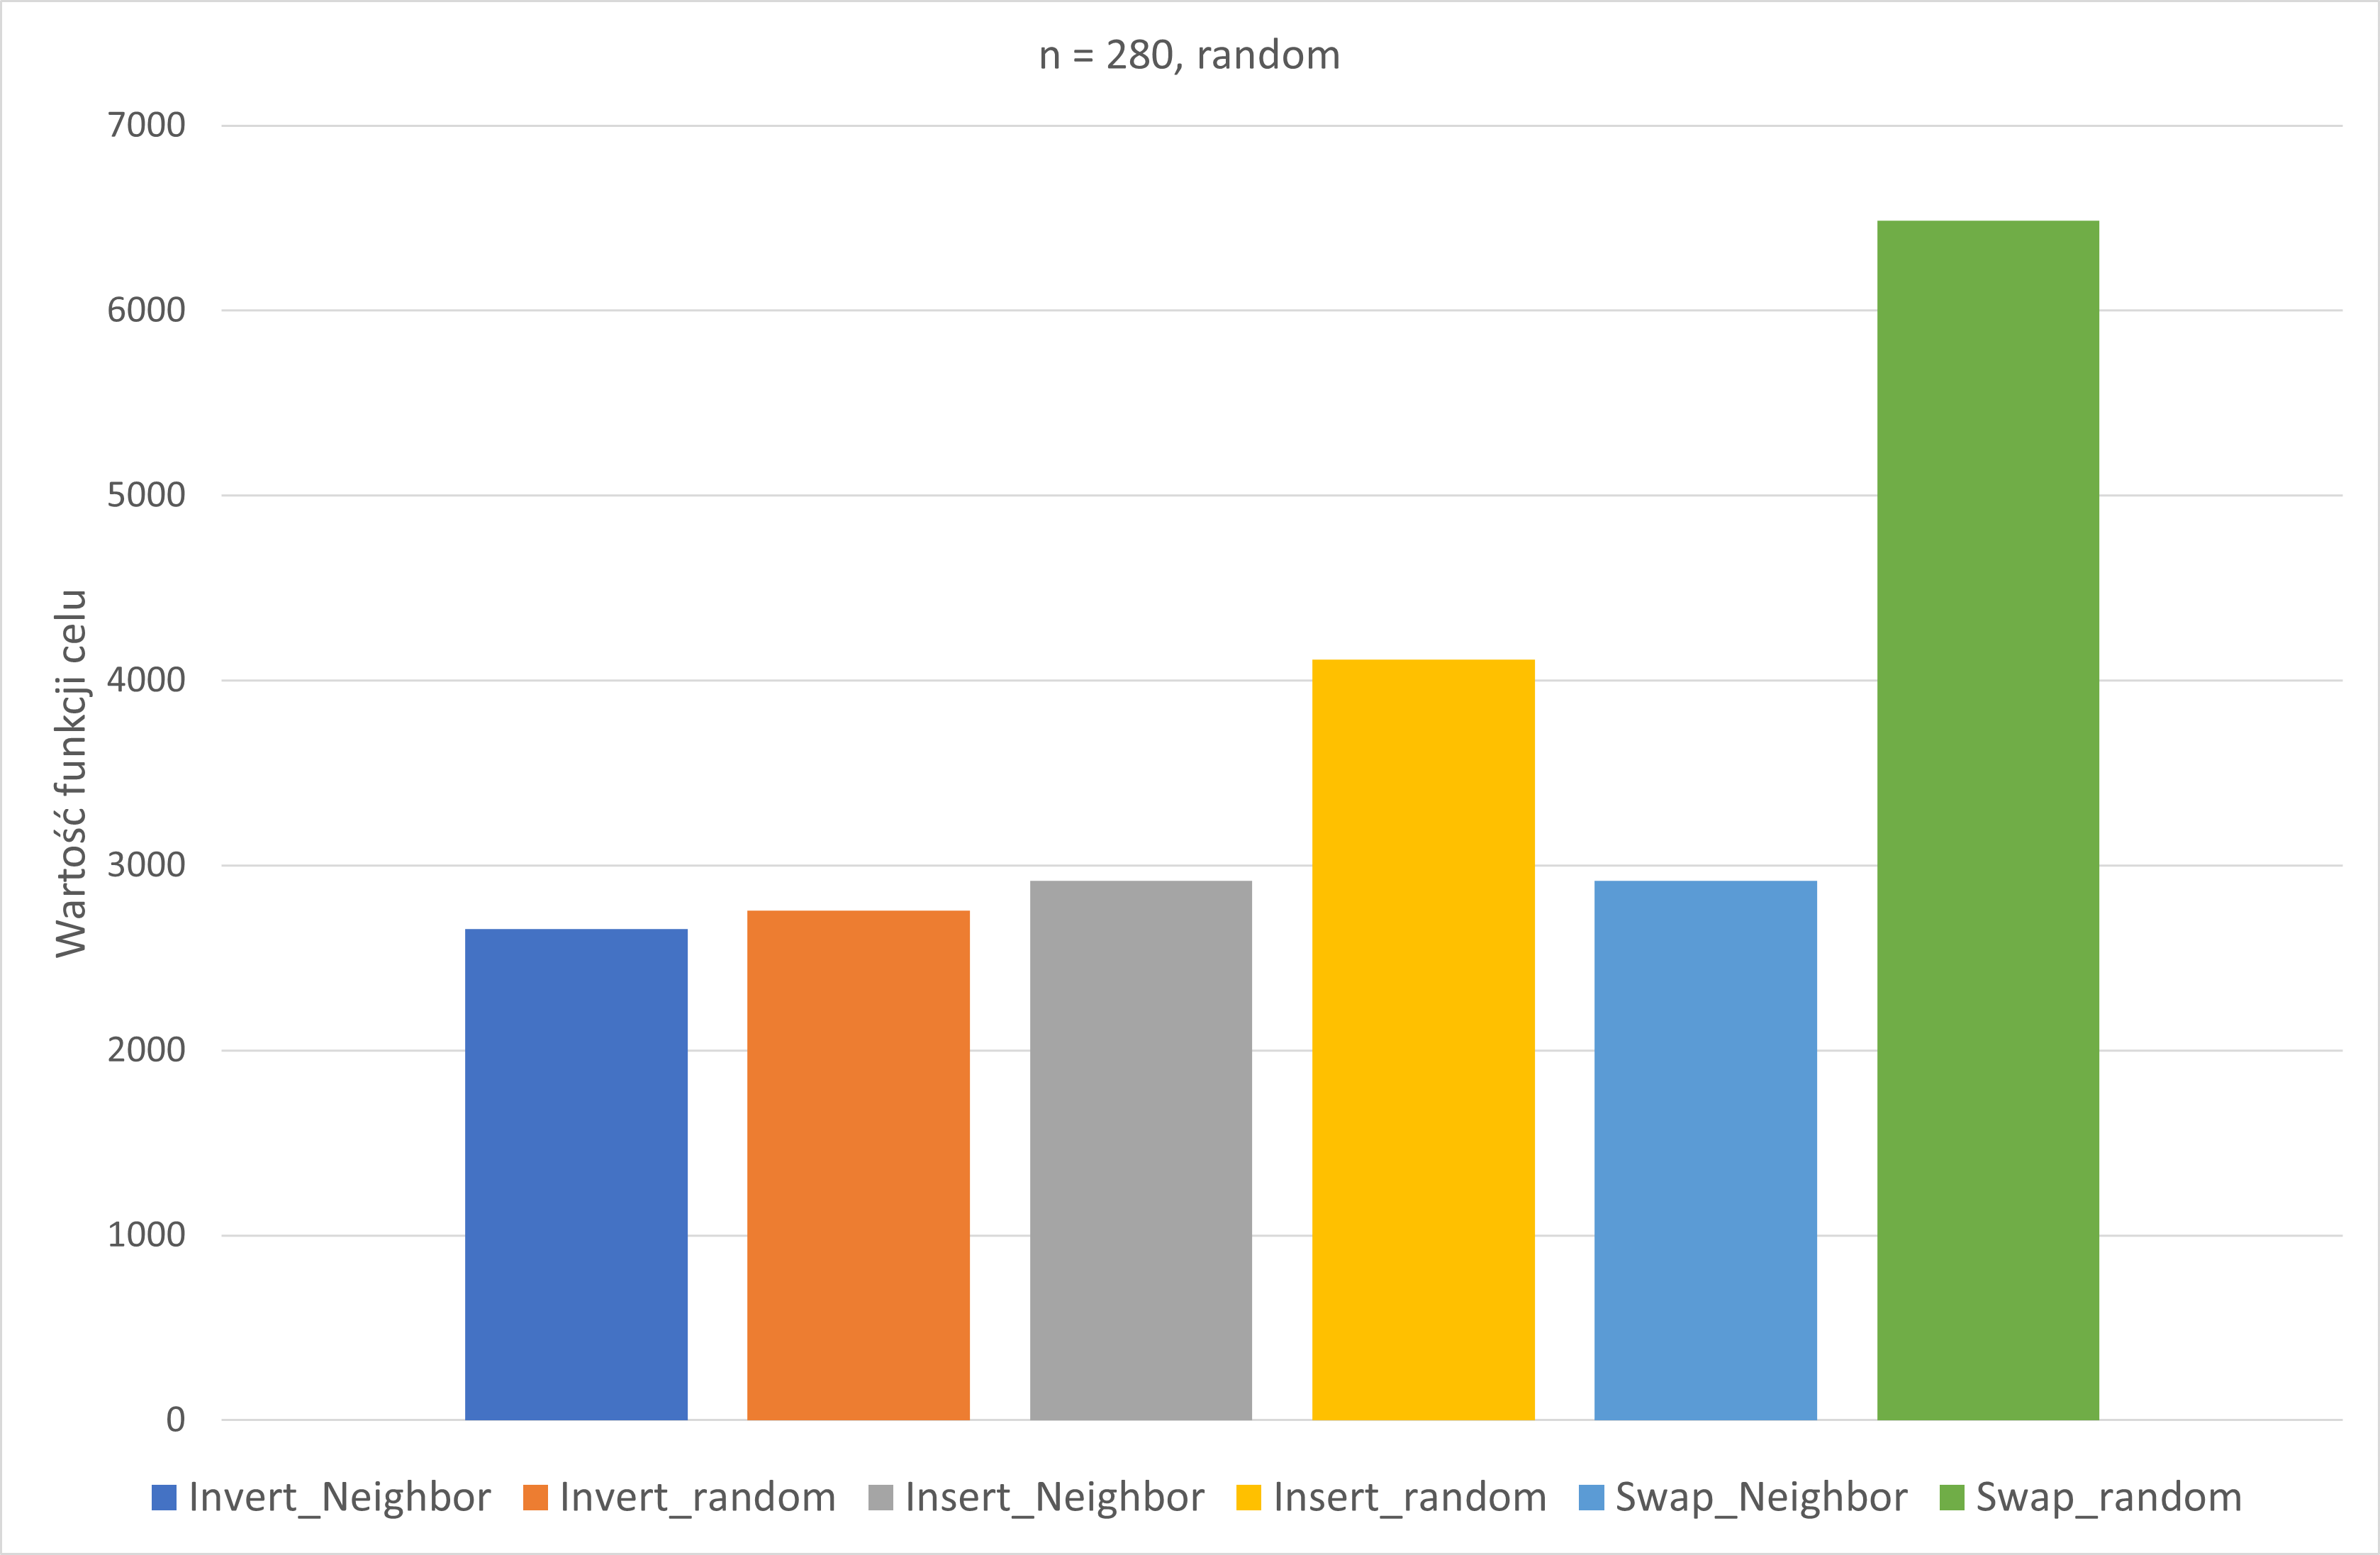
\includegraphics[scale=0.36]{280_rand}
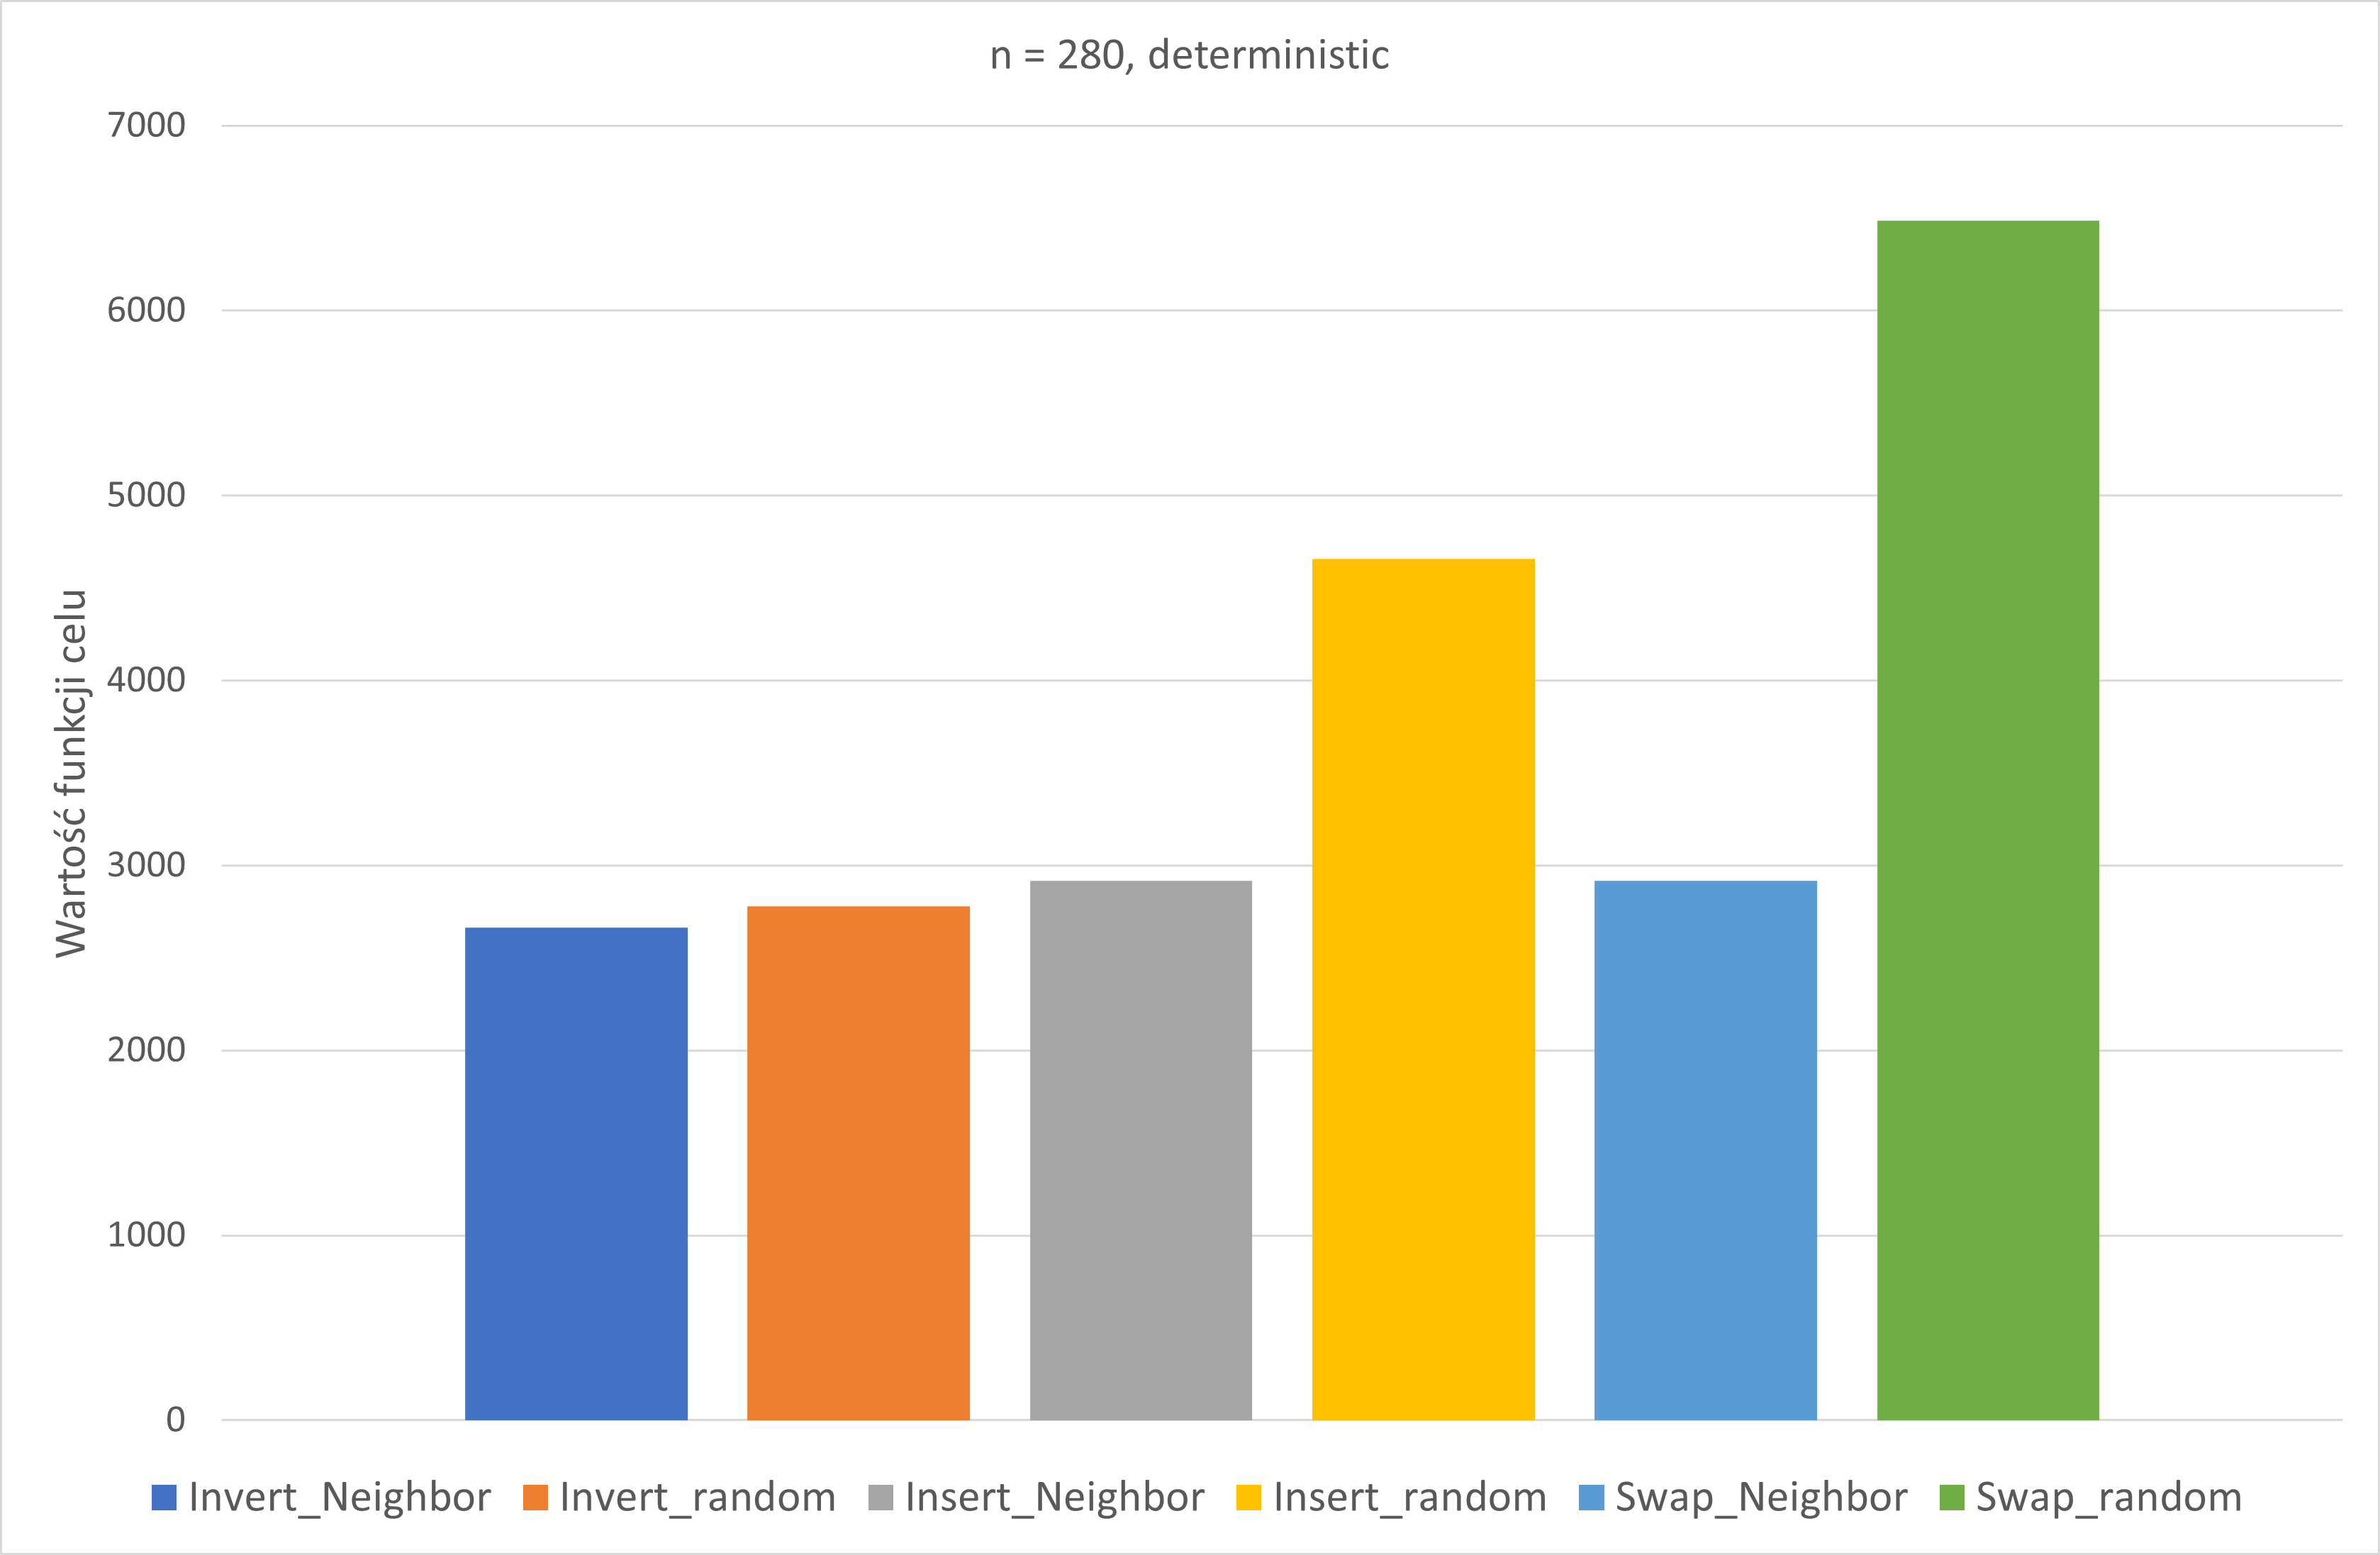
\includegraphics[scale=0.36]{280_deter}
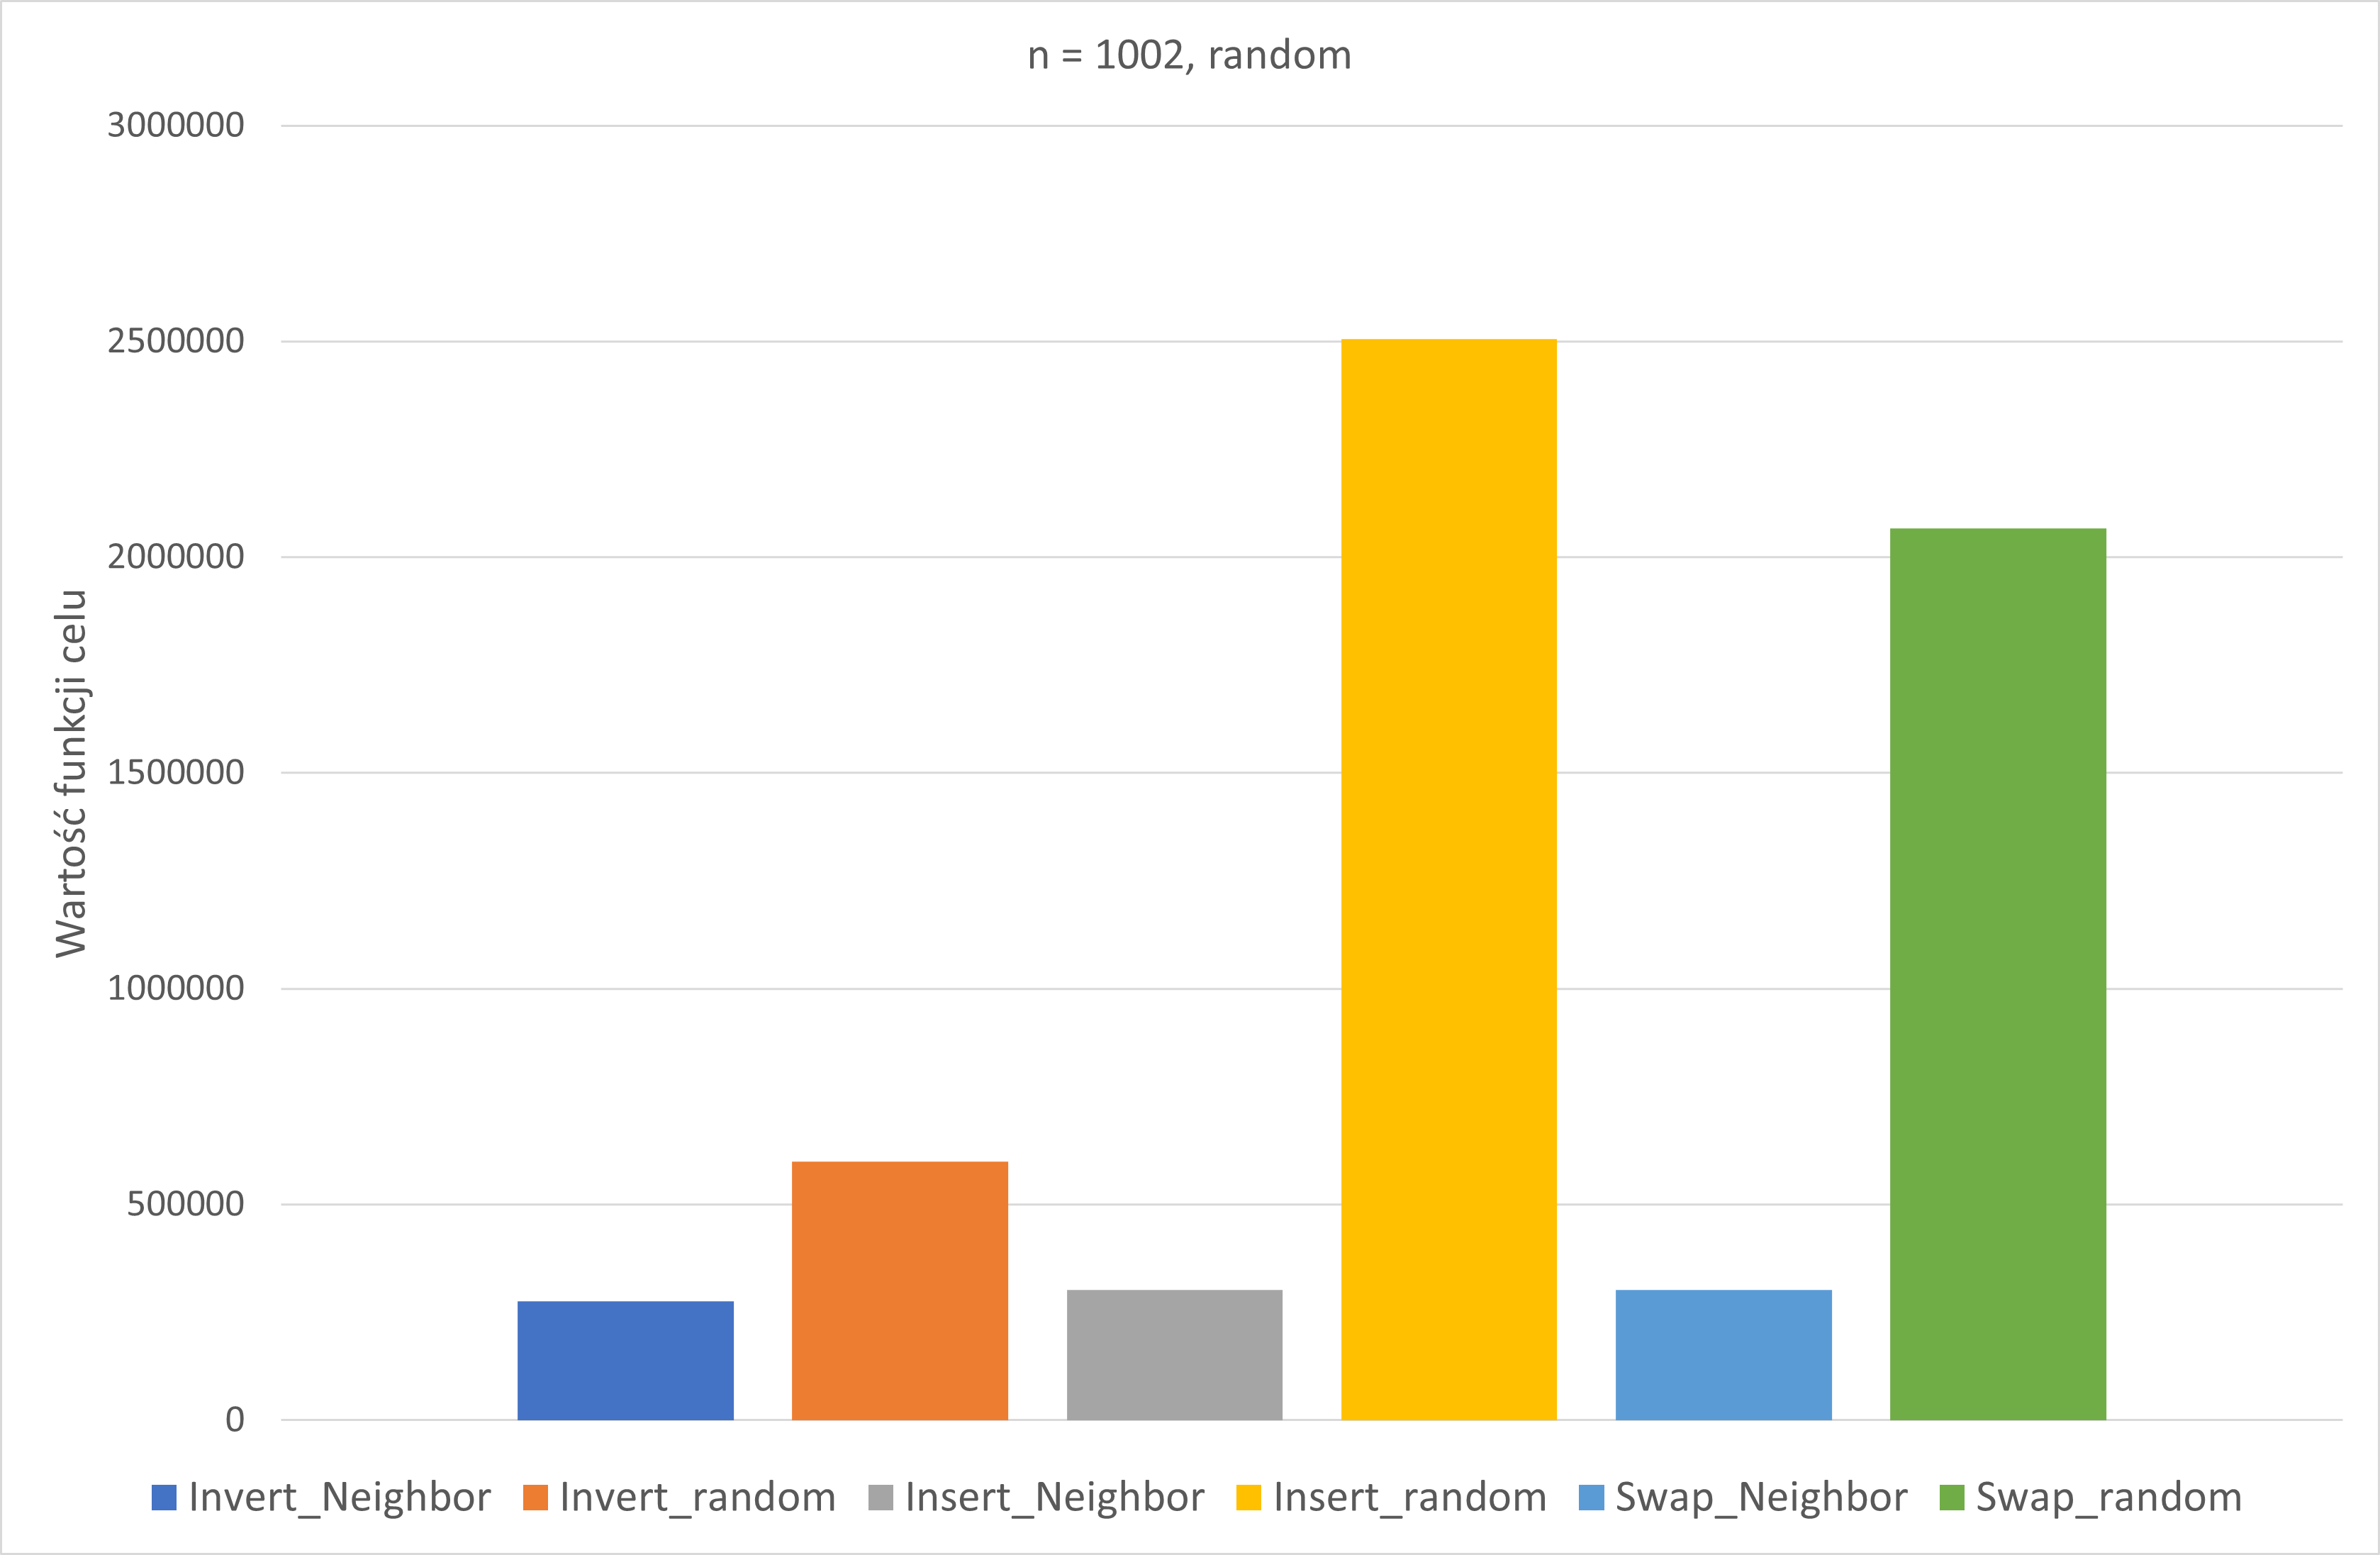
\includegraphics[scale=0.36]{1002_rand}
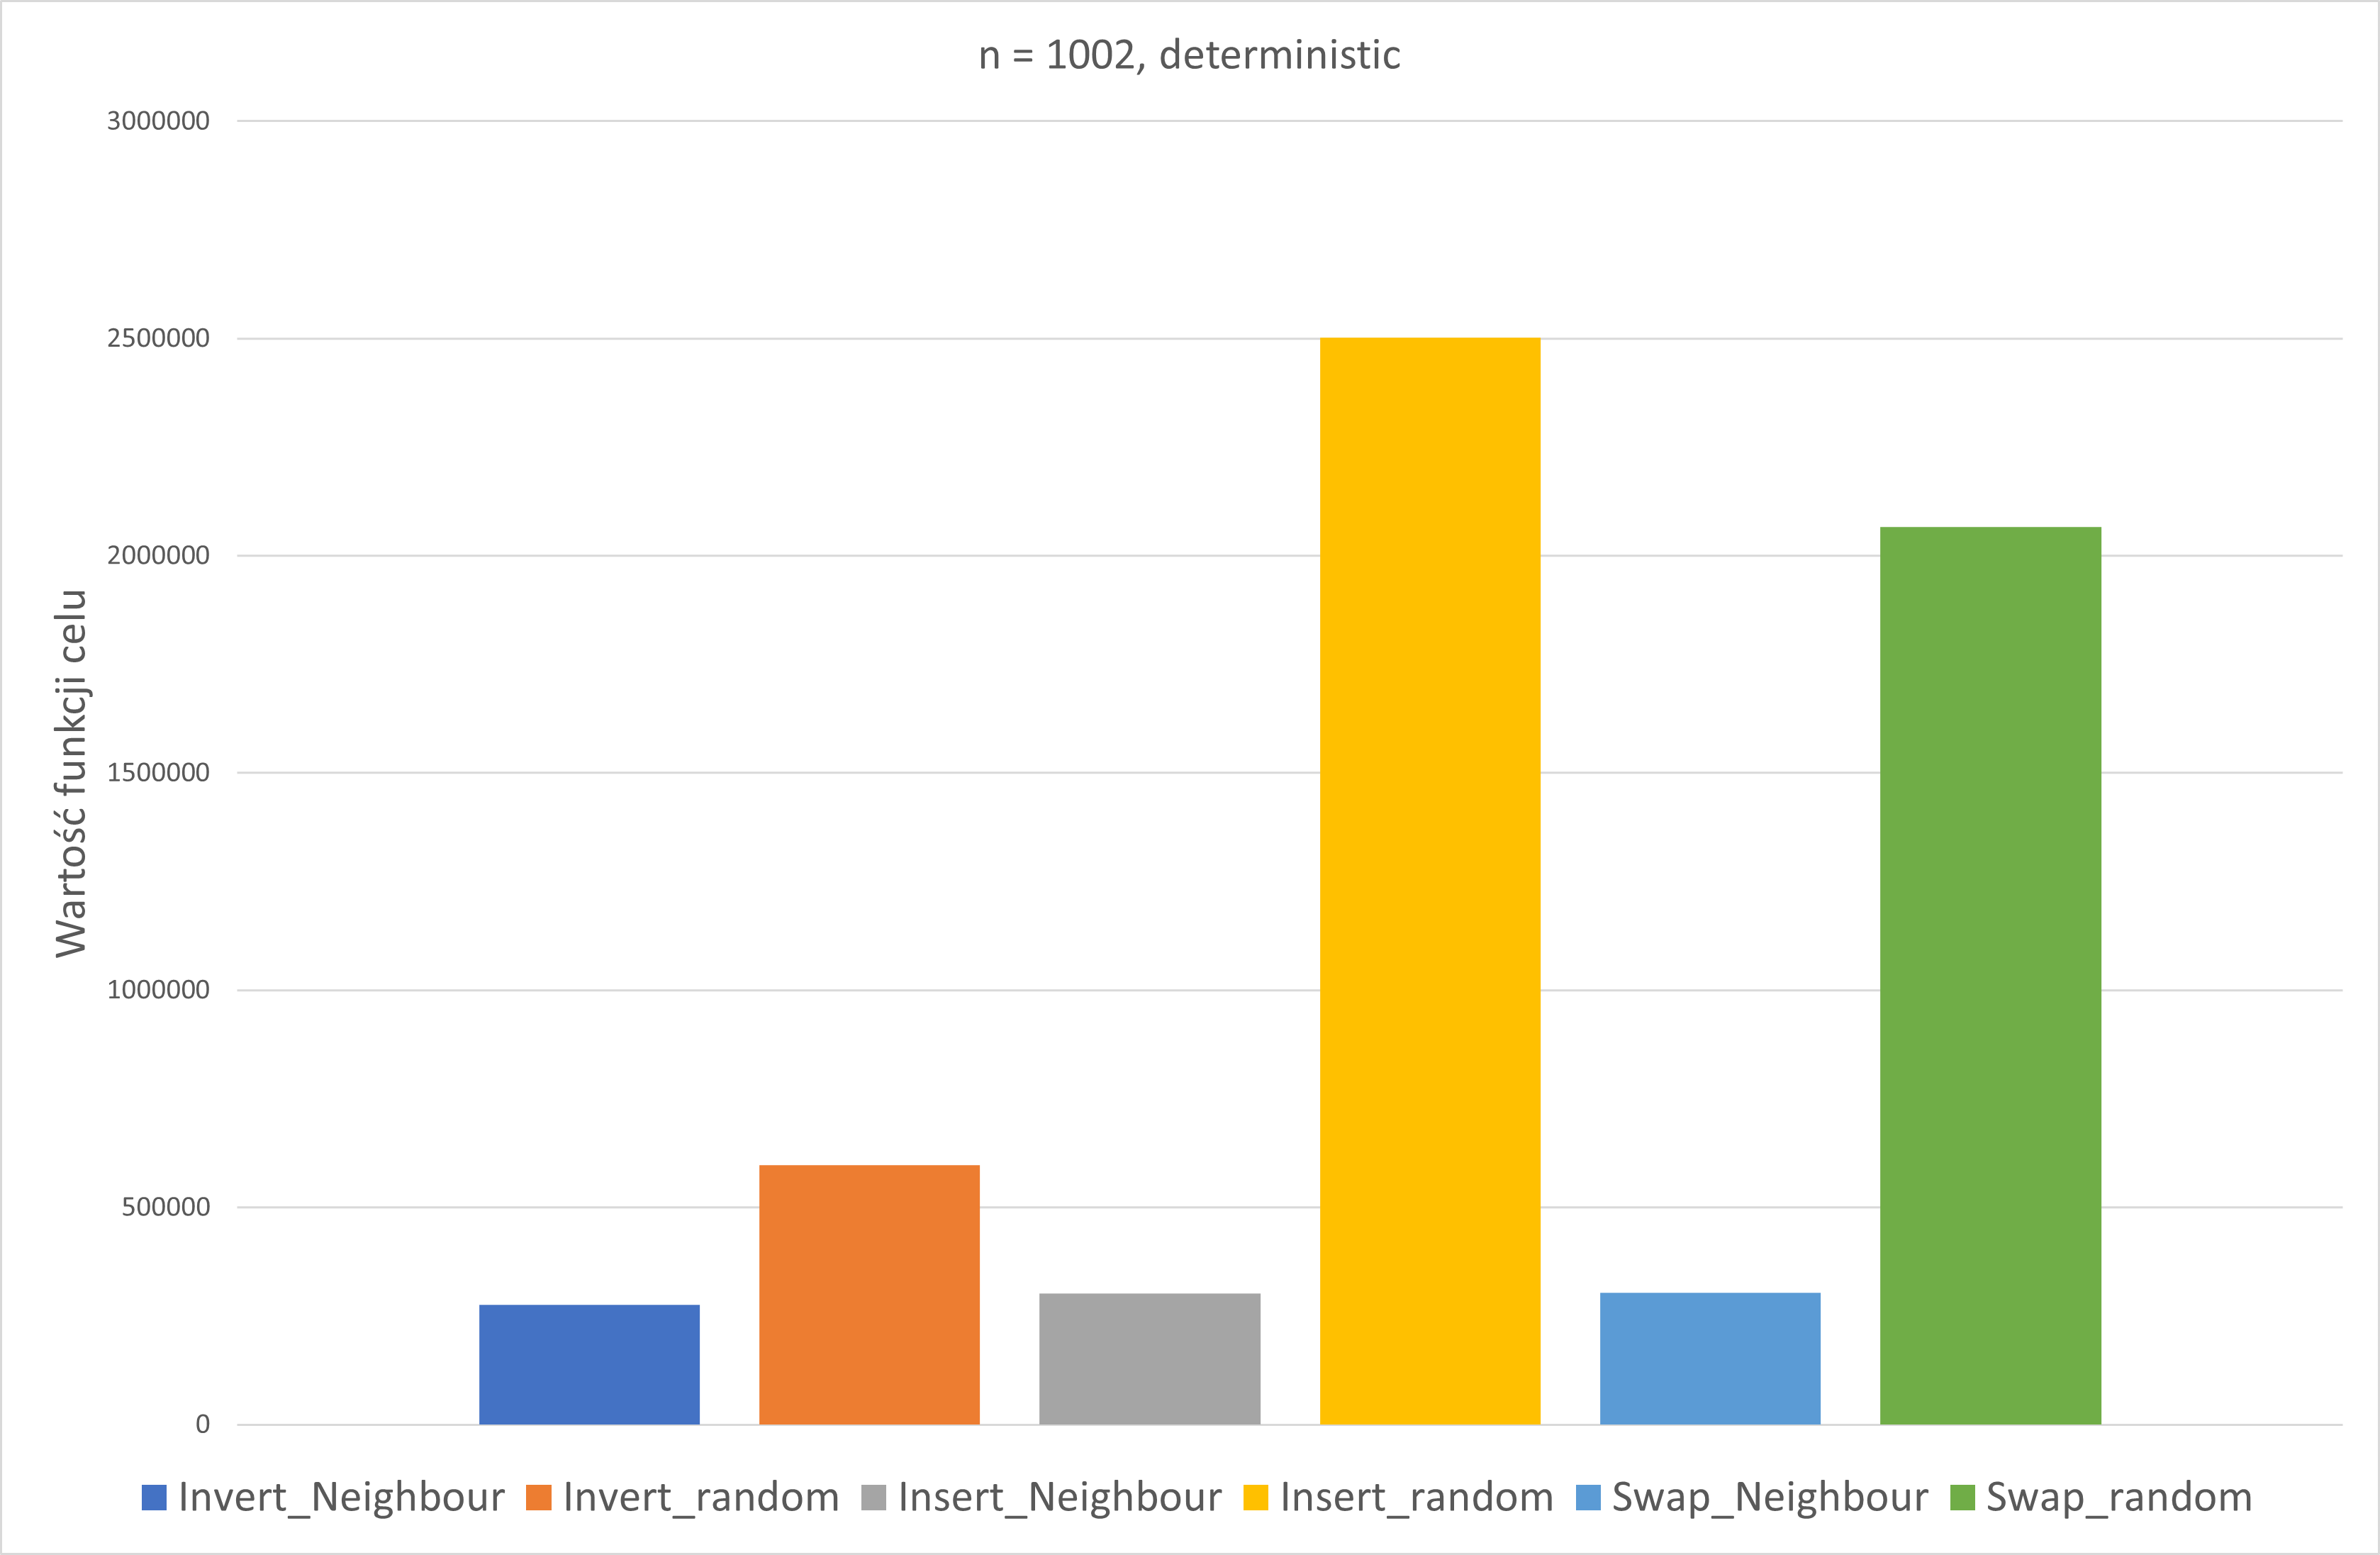
\includegraphics[scale=0.36]{1002_deter}

W obydwu wariantach operacji \texttt{kick} można zauważyć zbliżone wyniki przy wszystkich wielkościach problemu. Co więcej, wraz ze zwiększaniem się problemu bardziej klarownie widać różnice między wersjami. 
\begin{itemize}
	\item Początkowa trasa na podstawie Nearest Neighbour daje lepsze wyniki niż k-random
	\item Wszystkie otoczenia są porównywalne, najlepszy Invert, następnie Insert, najgorszy Swap
\end{itemize}


\subsubsection{Algorytmy uwspółbieżnione}

Uwspółbieżnienie zaimplementowano na zasadzie równoległego uruchamiania kilku instancji algorytmu \texttt{TABU-Search} jednocześnie. Z oczywistych względów nie testowano zachowania deterministycznej wersji algorytmu. Niestety, ta metoda uwspółbieżnienia nie dała dobrych rezultatów:

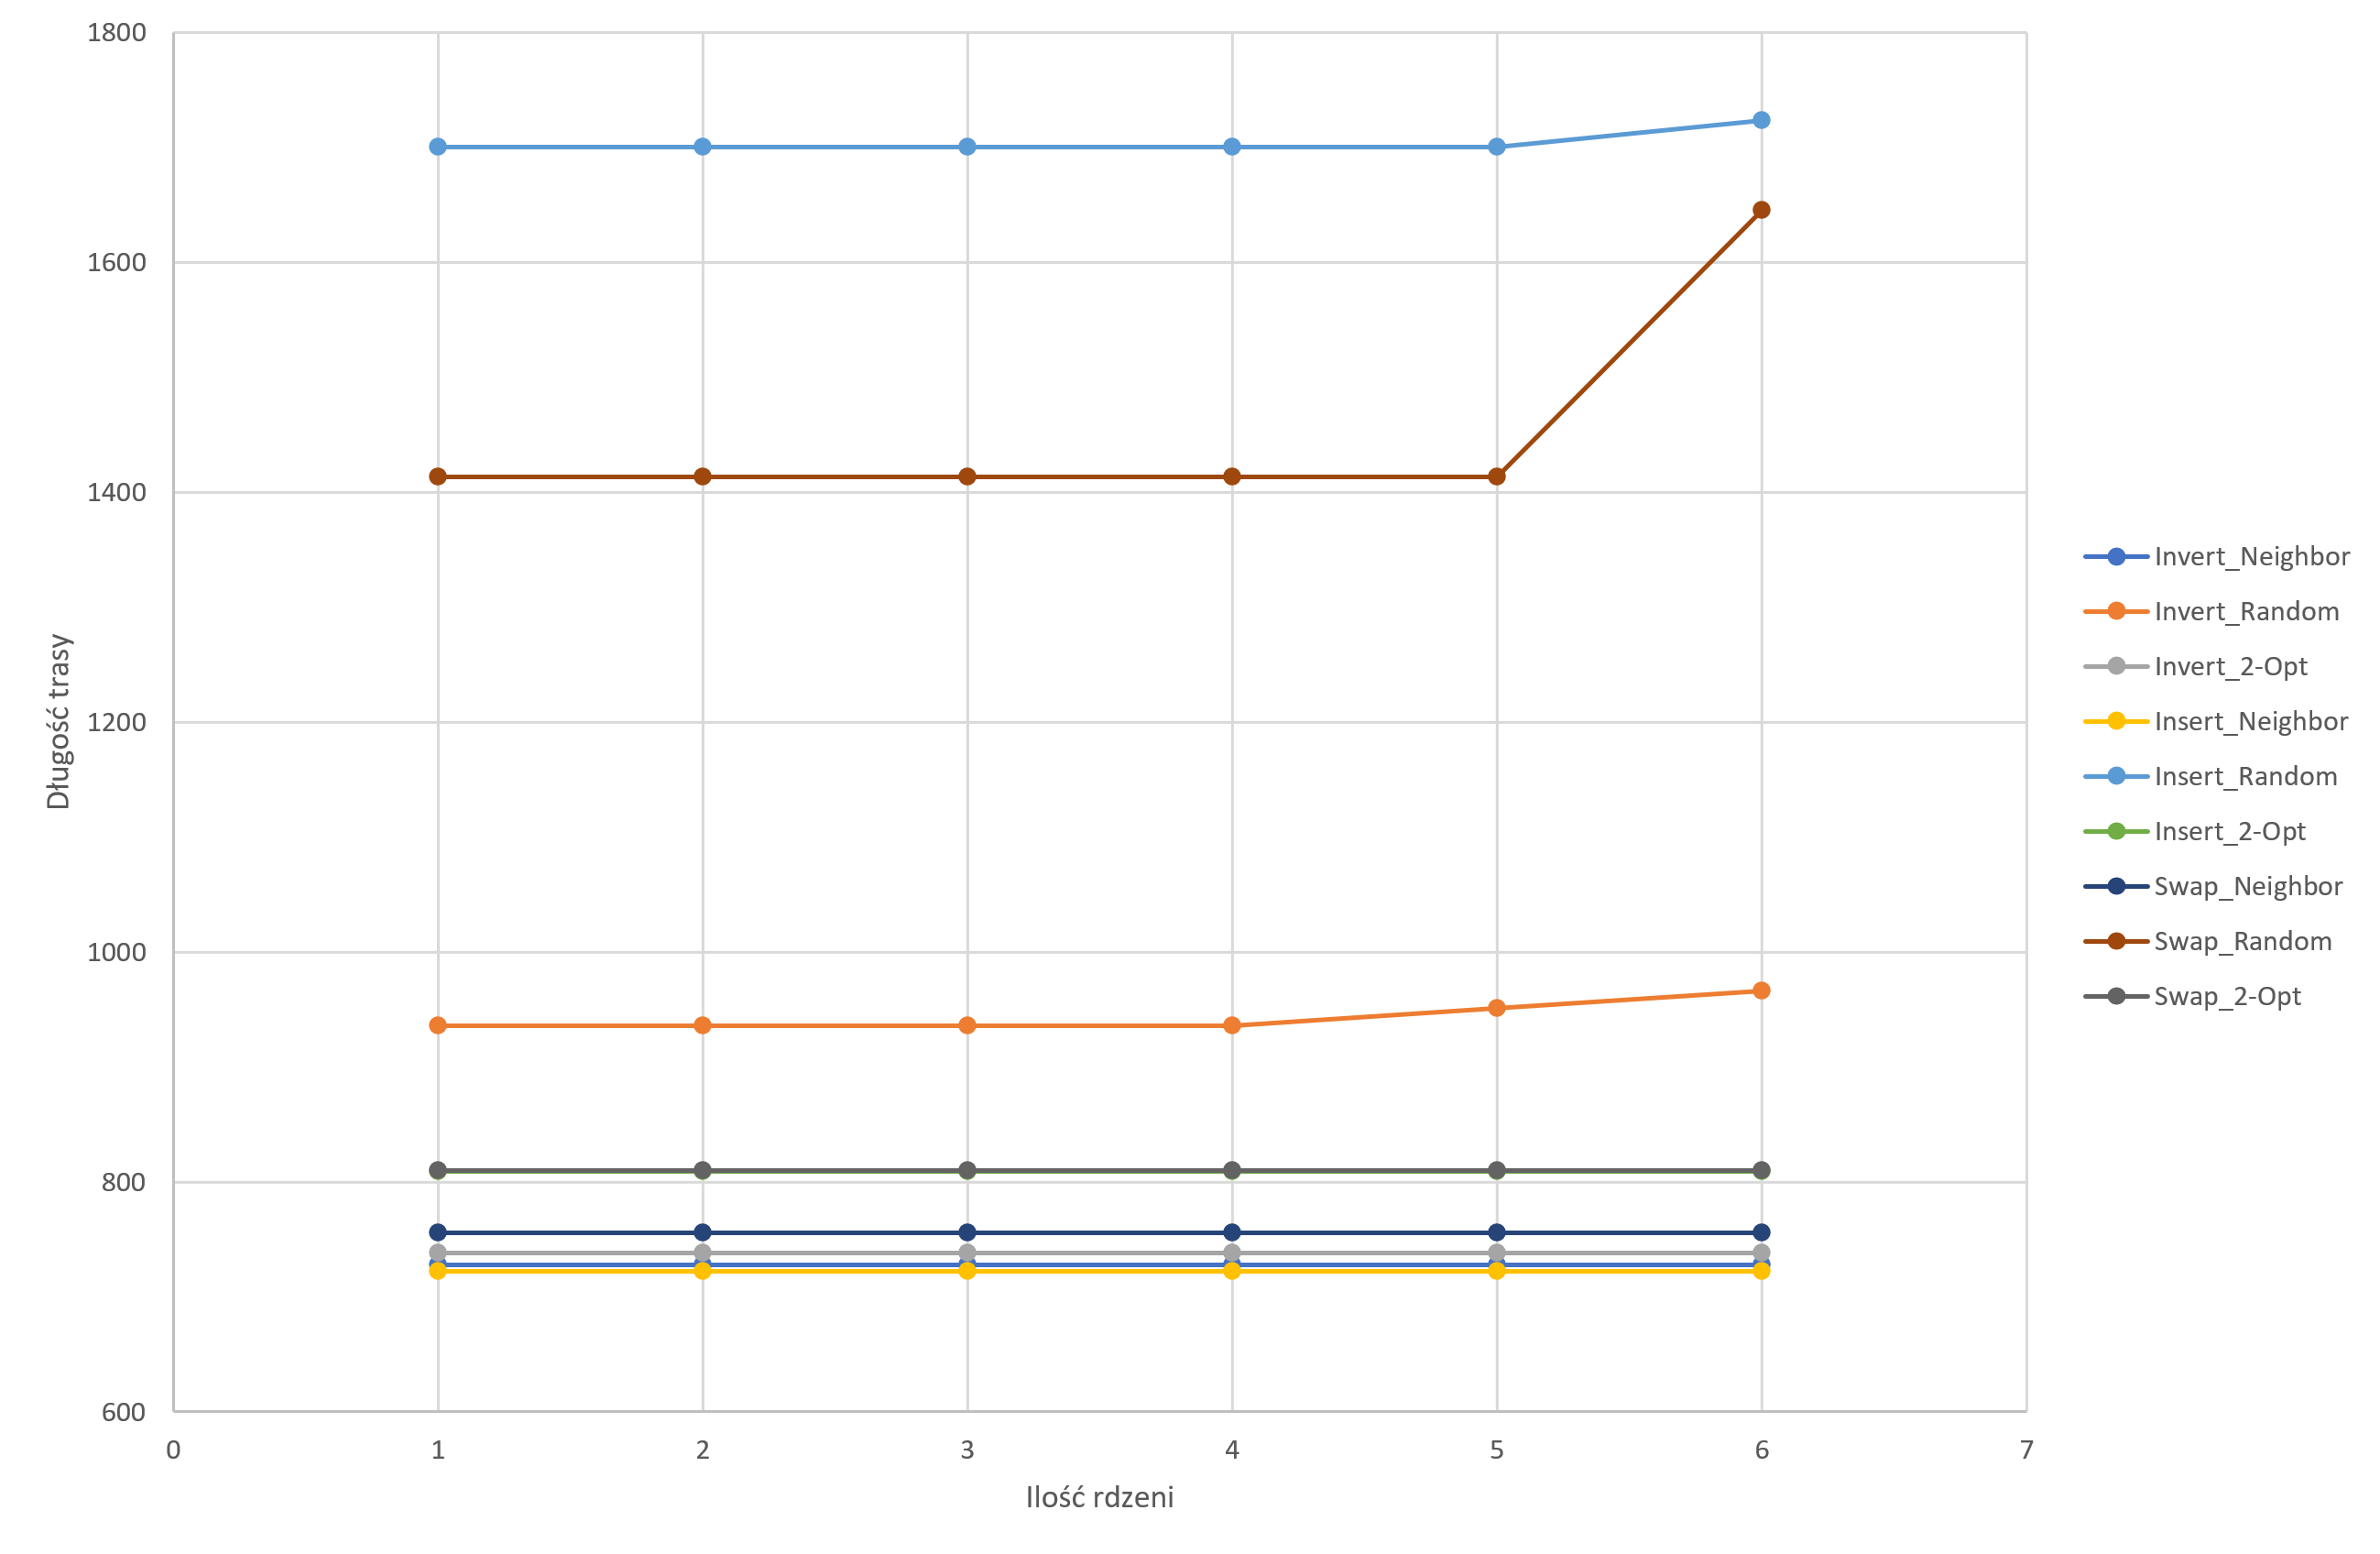
\includegraphics[scale=0.4]{parallel_n=70}

Dla każdego otoczenia i każdego rodzaju trasy startowej nie uzyskano w ten sposób polepszenia trasy.



\subsection{Wnioski}


\section*{Drobne uwagi}

\end{document}